\title{Automated Censorship Attack Rejection}
\author{
        Vitalik Buterin \\
        Ethereum Foundation
}
\date{\today}

\documentclass[12pt]{article}

\usepackage{graphicx}

\begin{document}
\maketitle
\begin{abstract}
Most research into blockchains assumes that the majority of miners or validators are honest, or at least are non-coordinating and either honest or economically motivated, and tries to prove claims taking these assumptions for granted. It is typically assumed that if 51\% of miners or validators actually are malicious and colluding, then nothing can be done to prevent the blockchain from being destroyed.

This paper is part of a line of research that seeks to challenge this assumption, showing that there are in fact ways that we can automatically detect and quasi-automatically recover from 51\% attacks, though usually at the cost of ``extra-protocol governance assumptions'' - that is, an assumption that the \textit{users} of a protocol can, in extremis, manually verify which of a set of competing chains launched what would intuitively be viewed as an attack, and choose the honest chain. The goal of this line of research is to \textit{minimize} the need for extra-protocol governance, including mathematically proving bounds on the number and scale of ``governance events'' that an attacker can trigger at a given cost, and \textit{standardize} its form, allowing it to be used for the specific purpose of detecting and rejecting majority-driven attacks while maintaining strong and credible norms that would make sure it continues to be difficult to abuse social coordination to trick a community into accepting chains that violate desired guarantees.

The main prior work in this direction is Casper [cite], which achieves the guarantee that even in the case of a 51\% finality reversion attack, the attacker can still be heavily penalized. Here, we seek to go further than finality reversion attacks and cover the other major category of 51\% attack: \textit{censorship}. We discuss the possibilities and limits of \textit{automated censorship rejection} - that is, the use of ``smart fork choice rules'' in blockchains that are aware of messages that have been broadcasted and that need to be included in the blockchain, and reject any chain that does not include these messages within some ``grace period''.
\end{abstract}

\section{Introduction}
One of the main classes of majority attack against blockchains is the \textit{censorship attack}: a majority attacking coalition builds a chain that refuses to accept transactions or messages that an ordinary validator, miner or client would accept, either depriving their victims of revenues from the consensus mechanism or depriving users of their right to get transactions included into the blockchain.

Unlike invalid block attacks or finality reversion attacks, which can both be detected by a purely passive client by means of a single non-interactive proof, censorship attacks are inherently more difficult to detect. This is because the definition of a censorship attack involves a listener (i) hearing about a message, and (ii) not taking an action based on that message that they should have taken, which inherently depends on events that have taken place in the past, which a client that is only online in the present can have no knowledge of.

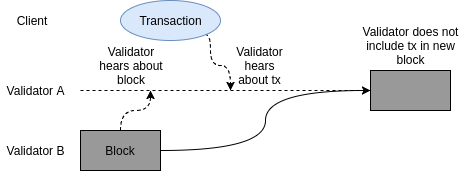
\includegraphics[width=400px]{Censorship1.png}

Most blockchain projects make no effort to even try to deal with the problem of majority coalition attacks such as censorship; an honest majority is usually one of the assumptions in any formal security proofs and models. Our goal is to see if we can go further.

\section{Forgiving Rejection}

For simplicity, let us assume that there exists a simple Nakamoto-style blockchain, where consensus is determined by the longest chain rule.

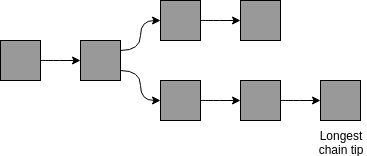
\includegraphics[width=400px]{Censorship2.png}

Suppose further that there is only one type of transaction. This type of transaction requires a very large amount of proof of work to create, for anti-denial-of-service reasons, and we make the computational assumption that there does not exist enough computing power in the world to create more valid transactions than a single node can verify as part of the process of verifying a block (we are deliberately very generous with assumptions at first to illustrate the basic principle).

Now, let us modify the Nakamoto fork choice rule with an additional rule: if a node sees a transaction X for the first time at time T, then starting from time T + 168 hours, it will reject all chains that do not include X. We assume that transactions are always re-broadcasted, so that all honest clients and miners see all transactions (this is a reasonable assumption because it is already the case with blocks).

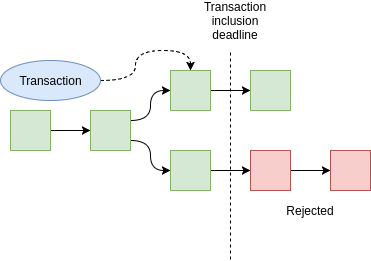
\includegraphics[width=400px]{Censorship3.png}
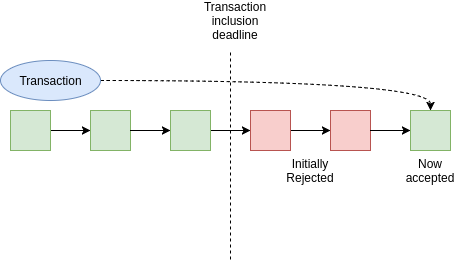
\includegraphics[width=400px]{Censorship3p5.png}

Notice that the primary guarantee of non-censorship is now met trivially. If a node sees a transaction X, then the blockchain that it accepts must, by definition, be a blockchain that includes X, at least after 168 hours. The harder claim to evaluate has to do with \textit{agreement}: that is to say, can we guarantee that a blockchain with miners running these rules will not permanently split?

Let us first suppose a synchrony assumption of one minute. Proof of work assumes a synchrony assumption implicitly, as if excessive network latency is permitted then it is quite easily possible for two chains to grow in parallel forever [cite 1], so this introduces no new assumptions. If this synchrony assumption applies both between miner and miner and between miner and client, then in the normal case no new risks are introduced: all miners will hear about all broadcasted transactions within one minute, miners include transactions immediately, and so analysis is identical to the standard Nakamoto case.

Now let us consider the possibility of \textit{temporary} 51\% attacks. Suppose that an extremely powerful miner broadcasts a block tree (that is, a chain or a diverging set of chains), and after this the miner's hashpower drops back to well below 51\%. For any given (block, transaction) pair, there is a maximum difference of two minutes in each client's perceived delay between the transaction and the block, and so it is very possible that some transaction was published (and seen by all clients) at time T, a chain not including that transaction published at time T + 168 hours - 30 seconds, with some clients perceiving the chain as having arrived before the 168 hour window and some clients perceiving the chain as having arrived after this window.

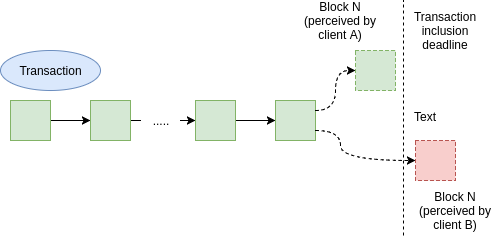
\includegraphics[width=400px]{Censorship4.png}

Consider the set of blocks which are considered "chain heads" by at least some honest miners (though possibly not all for temporal reasons). During every instant of time there is some probability that an honest miner will discover and publish a block that extends the one of these chain heads that is longer than all the others, and which includes every transaction that causes other miners to reject the block. The new chain head in this situation will be accepted by all clients and miners, and will be seen as taking precedence over all the others, and so all miners and clients will converge on it.

We can now weaken the synchrony assumption: suppose that only \textit{miners} have a guaranteed synchrony of one minute; \textit{clients} may log off for unboundedly long periods of time. Suppose that a client logs on after a very long time. They will then receive transactions that other clients heard earlier. Hence, they may accept chains that other clients reject (for example, if a transaction that was actually broadcasted 169 hours ago has not been included in some chain, the newly-online client will still accept that chain because they only saw the transaction much more recently), but they will under no circumstance reject chains that clients that have been online all along will accept.

If there is no 51\% attack going on at present, then by definition there is no longer chain than the chain that online clients and miners accept, and we know that the newly online client will also accept it. Now, suppose that there is an attack taking place. Then, it is already known from Nakamoto consensus research that the chains that different clients accept may be different, because 51\% attacks can cause persistent chain splits. The newly online client may well accept a chain that other clients reject. However, when the attack subsides, a chain that other clients accept will once again be the longest one, and so the newly online client will also accept it.

The algorithm achieves these properties because it is \textit{forgiving} - it accepts any chain that was censoring transactions initially, as soon as that chain stops censoring. However, the guarantee is very weak - it simply guarantees that clients will be on a chain that accepts transactions they know about, without any regard for how long they were censored in the meantime. It also assumes that the set of transactions that must be included is very small. Next, we will see to what extent we can expand and generalize these guarantees.

The arguments given in the previous section do not directly depend on any deep properties of Nakamoto consensus. \textit{Any} consensus algorithm that has some notion of a fork-choice rule can be used in its place. This includes GHOST [cite 2], and even partially-synchronous ``finality-bearing'' fork-choice rules such as the Casper fork choice rule.

\section{Unforgiving Rejection}

We can now try to strengthen the non-censorship requirement. The most natural use-case for strong anti-censorship protection is interactive verification - that is, mechanisms on blockchains where there exists some time period during which anyone can submit evidence that some fact F is false, and if no one submits this evidence during that period then it is assumed that F is in fact true. Mechanisms of this type include payment or state channels [cite 3], the Lightning Network [cite 4], Truebit [cite 5] or Plasma [cite 6]. This time period must have some definite length, and if a chain fails to include evidence within this length then it should be rejected \textit{unforgivingly} - that is, rejected forever, even if some child block later added to the chain accepts the transaction.

Preventing permanent disagreement in this model requires a hard synchrony assumption. Suppose that network latency is bounded by $d_n$. Suppose that, \textit{between validators}, the above algorithm runs with maximum permitted delay $d_v$, and rejection becomes \textit{unforgiving} if a transaction is not included in a chain within time $d_r$. When a transaction is sent, it will reach all validators within time $d_n$. By $max(d_v, d_n)$, honest validators will reject blocks not including that transaction, and so clients will not see any honest-node-supported chains not including the transaction after time $d_n + max(d_v, d_n)$. If we can count on the system reaching consensus within some time $d_f$ (eg. six blocks in typical proof of work chains), then this implies that as long as the consensus algorithm is functioning, there will not be problems as long as $d_r > d_n + max(d_v, d_n) + d_f$. For many interactive games, it is perfectly acceptable to set challenge periods several weeks long, and so we can see that setting $d_r$ to some length longer than a week may be an attractive option.

But what happens if there \textit{is} a 51\% attack? By adding this unforgiving rejection feature, we lose the ability to cleanly reject chains after successful 51\% attacks; instead, if a 51\% attack can persist long enough, it can create a \textit{permanent} chain split - or at least, a chain split that lasts until it is resolved via manual intervention.

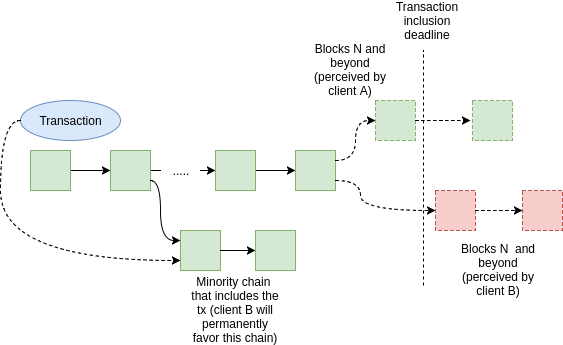
\includegraphics[width=400px]{Censorship5.png}

This is a genuine disadvantage for the security of proof of work chains that adopt this feature, albeit a surmountable one. Without unforgiving rejection, a 51\% attack on a proof of work chain would need to be permanent in order to cause a permanent chain split. With unforgiving rejection, the a 51\% attack that lasts one week is enough. However, the difference between the economic capacity needed to maintain a 51\% attack for two weeks and the capacity needed to maintain one forever is not that large.

In proof of stake, the disadvantage is even smaller, as a 51\% attack triggered even once may by itself be enough to create a permanent chain split, so by adopting unforgiving rejection we appear to lose nothing.

Even though off-chain governance - that is, clients manually selecting the chain that they perceive as being the honest chain and rejecting the attacking chain, is thus required to resolve 51\% attacks in both proof of work and proof of stake, by introducing unforgiving rejection we gain a major advantage. Because the censorship rejection mechanism forces a chain split, a censoring 51\% attacker no longer wins ``cleanly'' by default. Without automated censorship rejection rejection, the community must actively coordinate to reject a censoring 51\% attack chain. With rejection, at least some clients reject the censoring chain, and so there is no longer the pressure of a default in the attacker's favor - instead, the community must choose between two options of equal status, except that one is an attacking chain and the other is not, and so it seems much more plausible that the losing chain will win.

\section{Incentives in the Uncoordinated Majority Model}

There are two ways to analyze the incentives of automated censorship rejection. The first is to look at automated rejection \textit{between miners only}, and explore its game-theoretic properties in a model where all actors have minority hashpower. The second is to assume that the attacker has a great majority of all valdators (and we will assume that they are proof of stake validators, with some specific incentive rules), and try to prove that any harmful attack on the network will, in expectation, cost the attacker a substantial amount of money.

Pure forgiving rejection can be viewed as a Nakamoto blockchain where some blocks are, from the point of view of some miners, explicitly prevented from being the head, but a block on top of such a block can always be created which allows that chain to be the head again.

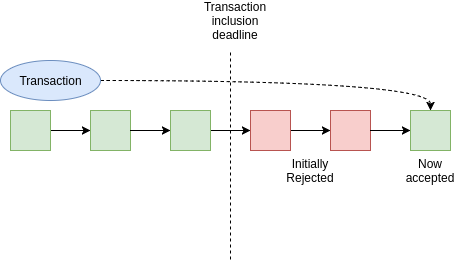
\includegraphics[width=400px]{Censorship3p5.png}

The question to ask is: is the rule of not mining on top of censoring chains, even if those chains are longer, incentive-compatible? The answer by itself appears to be no: mining a \textit{non-censoring block} on top of the longest chain is a dominant strategy over mining a block on top of the non-censoring chain. But then, the miners who create the censoring chain still get rewarded, and so there is no incentive to create a non-censoring block instead of a censoring block. Hence the entire scheme unravels.

But what if the scoring rule instead \textit{penalizes} censoring blocks - we have a rule that censoring blocks receive a score contribution of $\epsilon$, instead of a score contribution equal to the block's difficulty? Then, suppose that there is zero latency, so there is perfect shared knowledge on which blocks are censoring. In this case, this new rule is a deterministic monotonic fork choice rule as defined by Kroll et al [cite], and so it is a Nash equilibrium.

Suppose now that there is latency, and so sometimes miners will disagree over which blocks have the highest score. Mining is like a Keynesian beauty contest: one wins not by mining on what \textit{they} think is the main chain, but rather what they think \textit{others} will think is the main chain (where those others in turn are trying to guess what everyone else thinks is the main chain). With a fully deterministic scoring rule, the two perfectly align; with a subjective scoring rule they may not.

However, if we preserve the property that the block that a miner thinks is the head \textit{is much more likely than any other block} to be the block that other miners think is the head, then the game-theoretic argument remains effective. If each miner does not know their place in the distribution of network latency, then this property does hold; if all that each miner knows is that there are two groups of miners, A and B, with different views of what is the head, then they will a priori believe that they are more likely to be in the larger group. However, if miners \textit{can} see their network latencies and patterns of what blocks other miners create, then there will inevitably be strategies that are superior to the default one. So the incentive alignment is not perfect.

\section{Incentives in the Majority Attacker Model}

Now we can look at a malicious majority attacker. Our goal is roughly this: \textit{there must be a maximum ratio} between the amount of harm that (in expectation) an attacker does to the protocol and the amount of money that (in expectation) the attacker loses. To be able to talk about ``harm'' mathematically, we must define a ``protocol utility function''. Because chains that are censoring a transaction for more than two weeks cannot be valid by definition, and finality reversion attacks are currently out of scope, our protocol utility function need only consider one type of ``harm'' to the network: the chain split. Specifically, we can say $U = -\sum_{cs} (1 - win(cs))$: utility is the (negative, because we are measuring harm) sum, over all chain splits, of the portion of clients that were not on the winning fork, and thus had to manually switch chains.

We will then also use a simple proof of stake incentivization scheme: in a chain split, all validators are allowed to only support one fork (or else they get slashed), and on each fork, the validators who supported any other fork lose x\% of their deposits (we'll say 50\% for now). Let us now suppose that an attacker has 99\% of all deposits. They decide not to include a transaction until some time close to its latest allowed inclusion time. There are several possibilities, which we can describe by viewing the statistical distribution of the time delta that clients \textit{see} between the transaction being published and the transaction being included:

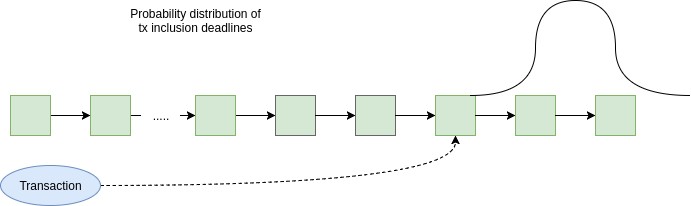
\includegraphics[width=400px]{Censorship6b.png}
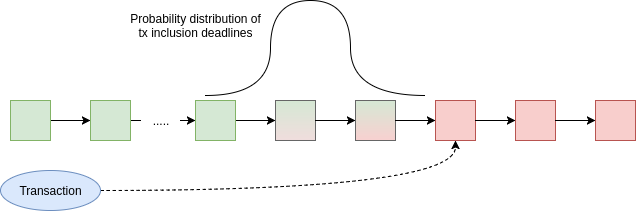
\includegraphics[width=400px]{Censorship6.png}
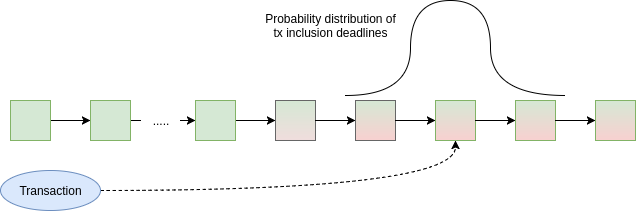
\includegraphics[width=400px]{Censorship6c.png}

In the first case, the transaction is delayed, and the attacker suffers no losses, but the delay is within tolerance and so no protocol guarantees are violated. In the second case, all clients reject the attacker's chain, instead going to a minority chain. The attacker loses money on the minority chain, and technically there is no harm to protocol utility. In the third case, half of the clients follow the minority chain and half do not. In this case, we can make the assumption that because the chain where the attacker loses money (instead of non-attacking validators) is more valuable, this chain will win. Utility is $-\frac{1}{2}$, and the attacker loses half of their money on the chain that the community accepts.

But there is also a fourth case:

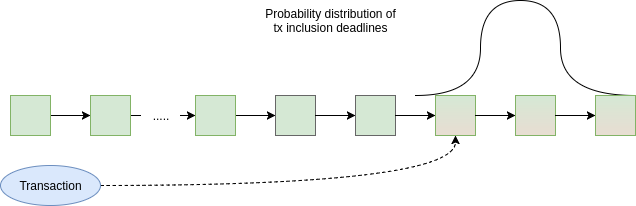
\includegraphics[width=400px]{Censorship6d.png}

Here, there is also a chain split, but only a very small portion of clients get split off from the majority chain. It is now much less plausible that this minority chain will win, and so we assume as a worst case scenario that the majority chain will always win in these cases. Utility is $-0.01$, and the attacker loses no money. This is a costless attack, which is what we want to avoid.

\section{Timelock Timers}

Let us now try a different approach. Suppose that instead of a hard timeout of one week, we have a different mechanism, based on timelock cryptography. A timelock function is a function $f(x) = y$ such that it takes some amount of sequential work to compute $f$ which cannot be sped up with parallelization, but where a result $(x, y)$ can be verified quickly. One example of a timelock function is Sloth [cite], roughly defined as follows:

\begin{verbatim}
def sloth(h, n):
    for i in range(n):
        h = pow(h, (p+1)/4, p)
        h += (1 if i % 2 else -1)
\end{verbatim}

Where $p$ is some prime. A result can be verified by running the same code, but with the two lines in the loop flipped, and the power replaced by a modular squaring; this is $O(log(p))$ times faster than the original computation. If a solution submitted is required to provide $n$ intermediate values, the result can be verified using $n$ threads in parallel, speeding verification up further.

We then have the following rule. When a transaction is included into a block with hash $h$, all clients start calculating $sloth(h, n)$ where $n$ is such that a result can be computed in one week. Once this value is computed, we \textit{retroactively} determine the maximum transaction inclusion window, as $168 - dist\_coeff * log_2(\frac{2^{256}}{sloth(h, n)})$ hours.

The intent is simple: make any attack that stands a chance of isolating a few users also have some chance of splitting the userbase in half. Now, we can describe the model as follows. Suppose that the distribution of clients' perceived time delta between transmission and inclusion has tails that are exponential or sub-exponential; that is, there exists some fixed $d$ such that if portion $\frac{1}{2^n+1}$ of the distribution is less than some time $t$, then half of the distribution is less than $t + n * d$. Note that this is a non-trivial assumption; for example, the normal distribution does \textit{not} satisfy this property, as the formula $\approx e^{-x^2}$ is \textit{super-exponential}. In the case that such a distribution exists, we will not be able to guarantee safety properties for the outliers. However, note that \textit{any} ``strong synchrony assumption'' as used in Byzantine fault tolerance literature implies a bounded distribution, which is inherently sub-exponential.

Let us set $dist\_coeff = d$. This now implies that any strategy which has probability $p_{2^{-n-1}}$ of ``forking off'' at least portion $2^{-n-1}$ of clients also has a probability of at least $p_{2^{-n-1}} * 2^{-n}$ of placing the distribution $n * d$ closer to the cutoff than expected, and thus forking off half of nodes. Thus, an attack which on average causes a utility loss $k$, on average causes a monetary loss to the attacker proportional to $k$.

\section{Proof of Work Timers}

The above approach inherently relied on a form of randomness, and a form of randomness that the attacker could not control. Another strategy is to use a different form of unpredictable randomness: proof of work. Here, we could have a rule that if, time $168 - dist\_coeff * n$ hours after a transaction, a client sees a proof of work solution that passes difficulty threshold $2^n$, then any blocks that come after that point are invalid unless they build on top of chains that include the transaction.

The problem is that a dishonest miner could publish a transaction at time $t_0$, then at time $t_0 + 168 - dist\_coeff * 50 - \delta$ publish a proof of work solution that passes the difficulty threshold $2^50$. A few seconds later they publish a block which includes the transaction. $\delta$ can be set in such a way that most nodes will \textit{perceive} $\delta < 0$, and so the proof of work solution is not sufficient, but a few nodes will perceive $\delta > 0$, and thus perceive the solution as being sufficient, and hence the transaction as arriving too late.

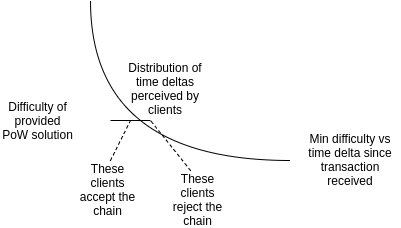
\includegraphics[width=400px]{Censorship7.png}

Suppose that an attacker has portion $h$ of hashpower. Once a transaction is published and not immediately included, there is a race to create a proof of work solution that triggers the timeout. Fraction $h$ of the time, the attacker succeeds first, and can accomplish the above attack cost-free. Fraction $1-h$ of the time, someone else succeeds first, and they can simply publish the solution. If the attacker has perfect control over the network, then they can still isolate a small portion of the nodes, but if they do not, then there will likely be a large split. Hence, if the attacker is not in control of most clients' network latency, then the cost of triggering disruption by not including a transaction is a cost of $1-h$.

Incentive compatiblity in the absence of a 51\% attacker is easy to show: because there are no 51\% attackers, all transactions will almost certainly be included well ahead of schedule, and so unforgiving rejection introduces no new obstacles. In the presence of a 51\% attacker, no strategy is reliably incentive-compatible, because in general for any strategy the attacker can always adopt a counter-strategy that penalizes validators which are detected to be engaging in that strategy. We assume that clients have a substantial preference for chains containing validators which do not have a track record of censoring them, and note that if the main chain is censoring then there is an incentive to build on the longest chain which is not censoring, and so an optimal honest validator strategy may in fact be something similar to forgiving rejection with a near-zero grace period.

\section{Censorship and Transaction Fees}

How do we extend this to the case where very large quantities of transactions get sent, and we want to ensure that fee-paying transactions get included? The challenge here is that users in the network may now send very large quantities of transactions, and there may not be enough block space to include all of them before the grace period expires; at least some users must be excluded. But what we *can* do is detect and prevent situations where higher-fee-paying transactions are excluded but lower-fee-paying transactions are allowed in.

Let us proceed as follows. The blockchain state contains a set of \textit{opportunities}. A \textit{transaction} consumes exactly one opportunity, and creates zero or more new opportunities. An opportunity could be a UTXO, an $(account, nonce)$ pair or one of many other schemes. We assume that the set of opportunities consumed by a transaction is statically determinable and unchanging, and the set of opportunities created by a transaction may be dynamic (i.e. dependent on the blockchain state at the time of transaction inclusion). Opportunities cannot be consumed more than once. A transaction also is seen as paying some \textit{fee level}, defined as total fee paid divided by blockchain space consumed, and fee, fee level and blockchain space are all statically determinable. Note that this is more restrictive than Ethereum, where blockchain space consumed and hence total fee are dynamic, and is more restrictive than Bitcoin, where transactions may consume multiple input UTXOs. The blockchain also contains some notion of a \textit{minimum fee level}, and constantly adjusts this fee level so that on average, blocks are half full. Fees equal to the fee level are destroyed; the surplus is given to validators.

A client keeps track of the set of all opportunities in all states that were received in the last several weeks (we assume that a block cannot build on top of a parent block that was seen a very long time ago; this can be accomplished with the same censorship rejection machinery that we use for transactions). For each opportunity, it keeps a map $opportunity \times timeslot \rightarrow transaction$, where a timeslot is a period of one hour during which a transaction could have been received, and the transaction stored is the transaction paying the highest fee that consumes that opportunity. When a node sees a block, it scans through all opportunities for all timeslots which are sufficiently far back that any transaction from that timeslot, and looks for any transaction that pays a fee higher than the minimum fee in the block that has not yet been processed. If such a transaction exists, then the block is rejected.

The map $opportunity \times timeslot \rightarrow transaction$ can be pruned and compressed. One can add a time requiring each transaction to have a maximum inclusion time, and if it is (legally) not included before then, then it can be ignored. This allows pruning old timeslots. Second, a transaction received in one timeslot can also replace transactions in later timeslots that pay lower fees; hence, representation can often be much more compact. In a worst case scenario a transaction sender can send a chain of transactions that pay progressively higher fees at progressively later times to try to consume a given opportunity, but this would only be possible during an active censorship attack.

\bibliographystyle{abbrv}
\bibliography{main}

\begin{itemize}
\item Casper is currently a work in progress. See https://medium.com/@VitalikButerin/minimal-slashing-conditions-20f0b500fc6c, https://github.com/ethereum/research/tree/master/casper4/papers and https://github.com/ethereum/casper for recent work.
\item Christopher Natoli and Vincent Gramoli, ``The Balance Attack'': https://arxiv.org/pdf/1612.09426.pdf
\item Aviv Zohar and Yonatan Sompolinsky, ``Fast Money Grows on Trees, not Chains'': https://eprint.iacr.org/2013/881.pdf
\item Jeff Coleman, ``State Channels: An Explanation'': http://www.jeffcoleman.ca/state-channels/
\item http://www.econinfosec.org/archive/weis2013/papers/KrollDaveyFeltenWEIS2013.pdf
\item https://eprint.iacr.org/2015/366.pdf
\end{itemize}

\end{document}
